\documentclass[11pt]{article}
%Gummi|061|=)
\title{\textbf{Rational fraction}}
\author{Nicolas}
\date{}
\usepackage{graphicx}
\usepackage{amsmath}
\begin{document}

\maketitle

\section{Intro}

We can deduce the particle paths (pp for short) from the velocity field using the kinematic equations for a particle in the flow:
\[
\begin{pmatrix}
	\frac{dx}{dt} \\
	\frac{dz}{dt} \\
\end{pmatrix}
=
\begin{pmatrix}
	u \\
	w \\
\end{pmatrix}
\]

Our problem is steady, so we can get rid of the time $t$ and express directly $z$ as a function of $x$ 
\[
\frac{dz}{dx}(x) = \frac{w(x, z)}{u(x, z)}
\]
This ODE may seem "easy" to solve, but I can't figure it out, even in the following simple case, where $u$ and $w$ are rational fractions of $x$ and $z$:
\[
 u =
 \left(
 \alpha 
 +\frac{2 (\alpha -1) z (W-x)}{H x}
 \right) 
 \left(
 u_F
 -\frac{(2 n+1) U x}{(2 m+1) (2 m+2 n+1) (W-x)}
 \right)-u_F
\]

\[
 w = 
 \frac{z \left(\frac{(2 n+1) U (x (\alpha  H-2 (\alpha -1) z)+2 (\alpha -1) W z)}{(2 m+1) (2 m+2 n+1)}-\frac{(\alpha -1) uF z (W-x)^2}{x}\right)}{H^2}
 \]
 
 
\section{Particle paths}

The idea is to deduce the velocity field from the prescribed pp, instead of doing the contrary.
Our first job is then to build a realistic set of pp. 
In other words we would like to find a set of $z_a(x)$ where $a$ is parameter classifying the pp.
Given the shape of the wanted particle paths, it seems to be easier to construct $x_a(z)$ rather than $z_a(x)$.
First we will define the parameter $a$. $a$ could be the height of the pp infinitely away form the head of the flow: $a = \text{lim}_{x \rightarrow -\infty} z(x) \doteq z_\infty$. We could also decide that $a$ will be the $x$ coordinate of the pp at which it "goes back" (\textit{ie} at the point where $dz/dx = - \infty$). 
Let's call this point $x_0$.

I have a good feeling about this function:
\[
z(x; x_0, z_\infty, z_0) = z_0 + (z_\infty - z_0) \sqrt {\text{tanh} (-x + x_0)}
\]

Indeed we have 
\[
\begin{matrix}
	\lim_{x \rightarrow -\infty} z = z_\infty \\
	z(x_0) = z_0 \\
\end{matrix}
\]
as expected. For now $z$ is a function as 3 parameters, but only one, $a$, is needed.
Let's for example express $z_\infty$ and $z_0$ as functions of $a = x_0$. I choose
\[
\begin{matrix}
   z_\infty(x_0) = \text{tanh}(-1/x_0) \text{ if } z > z_0 \\
   z_\infty(x_0) = 1 - \text{tanh}(-1/x_0) \text{ if } z < z_0 \\
   z_0(x_0) = \frac{1}{2} \text{tanh}\left(\frac{-x_0}{x_0+1/\text{arctan}(1/2)}\right) 
\end{matrix}
\]

This gives us the following pp:

\begin{figure}[htp]
\centering
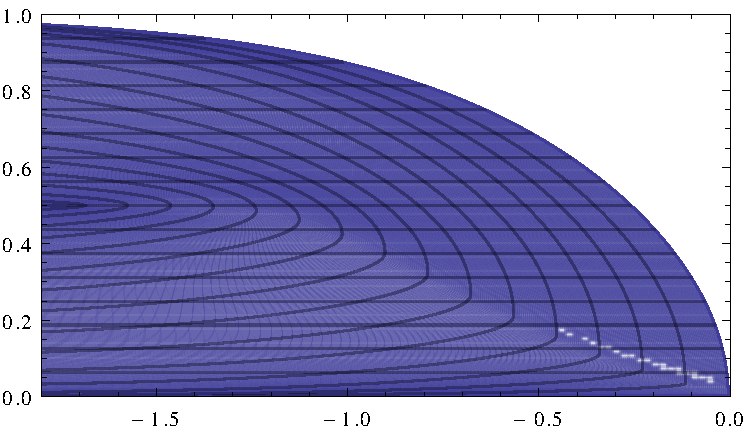
\includegraphics[scale=0.9]{remap_particle_paths.pdf}
\caption{Particle paths}
\label{}
\end{figure}

Note that $x_0$ varies from $0$ to $-1/\text{arctanh}(1/2)$ when $z_\infty$ goes from $0$ to $1/2$ (or from $1/2$ to $1$).
Therefore the pp "go back" to $x = -\infty$ only close to the head, in the finite region of space $[-1/\text{arctanh}(1/2);0]$.
I tend to think that the same thing happen with the velocity field of the flume paper, but this is only my feeling!

\section{Velocity field}

These pp seem rather similar to the one given by the velocity field used in the flume paper.
Now our job is to derive the velocity field corresponding to these new pp, and to inject it into our numerical solver to check if the desired spiralling structure will appear.

We have
\[
\frac{w}{u} = \frac{dz}{dx} = -\frac{(z_\infty - z_0)\left(1-\text{tanh}^2(-x+x_0)\right)}
		{2\sqrt{\text{tanh}(-x+x_0)}}
\]
Note that 
\[
\begin{matrix}
w  \xrightarrow[x \rightarrow -\infty]{} 0 \\
u  \xrightarrow[x \rightarrow x_0]{} 0
\end{matrix}
\]
as expected.
$w/u$ does not seem to depend on $z$, but recall that $z_\infty$ and $z_0$ are functions of $x_0 = x_0(x,z)$.
It is trivial to express $z$ as a function of $x$ and $x_0$, or $x$ as a function of $z$ and $x_0$:
\[
\begin{matrix}
z(x, x_0) = z_0(x_0) + (z_\infty(x_0) - z_0(x_0)) \sqrt {\text{tanh} (-x + x_0)} \\
x(z, x_0) = x_0 - \text{arctanh} \left[ \left( \frac{z - z_0(x_0)}{z_\infty(x_0) - z_0(x_0)} \right)^2 \right]
\end{matrix}
\]
However, expressing $x_0$ as an explicit function of $x$ and $z$ seem difficult.
Therefore it seems unlikely that we can have an explicit expression for $u$ and $w$ using these pp.
\end{document}
